El modelo cinemático desarrollado en la sección
 fue implementado en MATLAB
para evaluar el comportamiento del sistema.
Este simulador es capaz de calcular los cambios en 
la dimensión de cada elemento de movimiento del sistema
para lograr que la plataforma móvil 
llegue a la posición deseada.

El simulador cuenta con una interfaz gráfica que permite la 
evaluación de coordenadas y orientación de la plataforma.
Es posible especificar posiciones deseadas y 
los parámetros de movimiento del robot como lo son la
longitud de cada pistón y la dimensión de la base y 
plataforma del sistema.

\begin{figure}
 \centering
 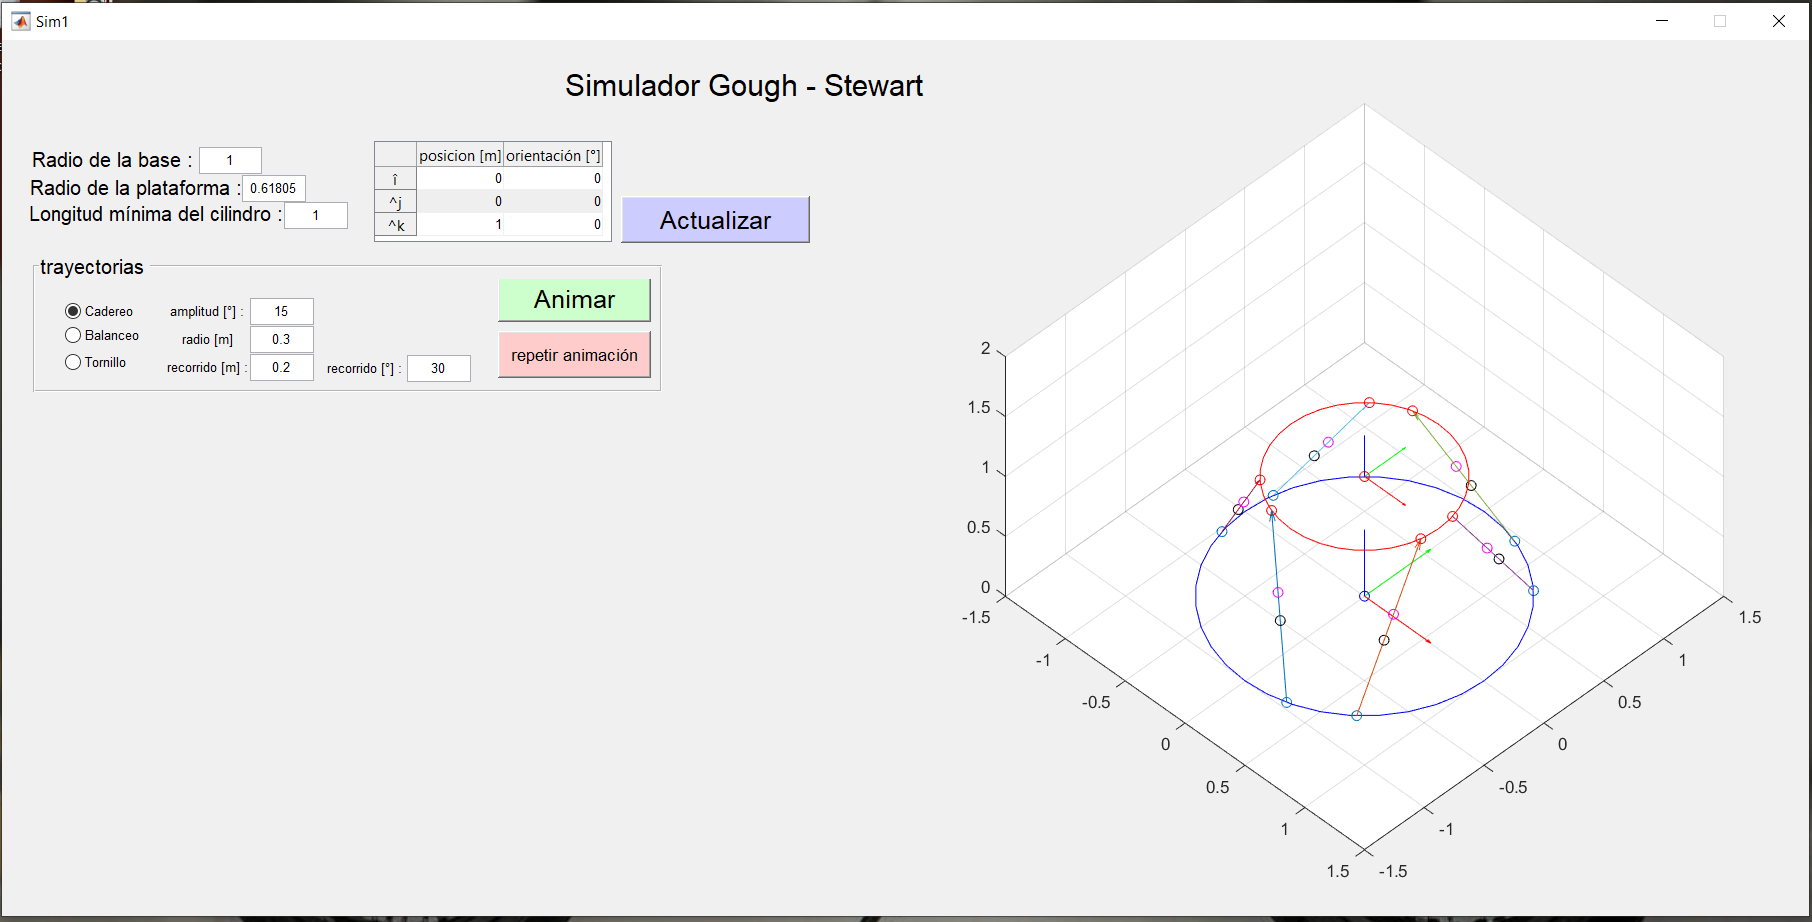
\includegraphics[scale=0.2]{img/principal.png}
 % principal.png: 1812x922 px, 120dpi, 38.36x19.52 cm, bb=0 0 1087 553
 \caption{Interfaz gráfica del simulador.}
 \label{fig: GUI}
\end{figure}


El simulador determina si la posición y 
orientación introducidas en la interfaz gráfica
es realizable con los parámetros especificados para
el robot. Para llegar a este resultado, el simulador realiza
las siguientes instrucciones:

\begin{itemize}
 \item Obtener la posición de cada junta de la base,
 con respecto al centro de la base.
 \item Obtener la posición de cada junta de la
 plataforma móvil con respecto a la base y tomando
 en cuenta la posición deseada.
 \item Procesar las coordenadas de cada elemento para 
 obtener los vectores que representan cada pistón.
 \item Evaluar si la posición deseada excede las 
 limitaciones físicas del sistema como exceder la 
 extensión o compresión máxima de algún pistón.
 \item Enviar mensajes de error si es necesario.
 \item Graficar los datos obtenidos, en caso de ser una
 posición factible.
 \item Ejcutar instrucciones adicionales 
 de la interfaz gráfica.
\end{itemize}

El simulador también es capaz de producir animaciones del 
movimiento de la plataforma y exportarlas como 
archivos MP4.
